\documentclass[11pt]{article}

%%%%%%%%%%%%%%Include Packages%%%%%%%%%%%%%%%%%%%%%%%%%%
\usepackage{xcolor}
\usepackage{mathtools}
\usepackage[a4paper, total={6in, 8in}, margin=1.25in]{geometry}
\usepackage{amsmath}
\usepackage{amssymb}
\usepackage{paralist}
\usepackage{rsfso}
\usepackage{amsthm}
\usepackage{wasysym}
\usepackage[inline]{enumitem}   
\usepackage{hyperref}
\usepackage{tocloft}
\usepackage{titlesec}
\usepackage{colortbl}
%%%%%%%%%%%%%%%%%%%%%%%%%%%%%%%%%%%%%%%%%%%%%%%%%%%%%%%%



\begin{document}
\Large \noindent \textbf{Physics 5C Discussion (Worksheet 1)}\\
\normalsize
Department of Physics and Astronomy, UCLA\\

\noindent TA: Jinyan Miao (jnmiu@ucla.edu)\\
Office hours: Thursday 2:30 - 4:30 PM (PST) over Zoom \\
Zoom ID: 963 5916 9873 (passcode: hiJinyan)\\
Click for the \href{https://ucla.zoom.us/j/96359169873?pwd=05p7ssCPwTbl8KfxoBNCOuaIbt68jW.1}{\underline{Zoom link}} and \href{https://sites.google.com/umich.edu/jmiu/worksheets}{\underline{solutions to the worksheets}}.\\
\noindent\rule{8cm}{0.4pt}\\

\noindent\textbf{Problem 1:} In this class, you will see two-dimensional and three-dimensional vectors. Two-dimensional vectors lie on a plane and are usually denoted as $\vec{v} = (v_x,\,v_y)$ in component form. Interchangeably, we can also denote a two-dimensional vector using its angle $\theta$ (measured from the positive direction of the $x$-axis) and magnitude $v$. The formulas that you can use to switch between the two notations are
\begin{align*}
v_x = v\cos(\theta)\,,\qquad
v_y = v\sin(\theta)\,,\qquad
v = \sqrt{v_x^2 + v_y^2}\,,\qquad
\theta = \arctan\left(\frac{v_y}{v_x}\right)\,.
\end{align*}
In Physics 5A, we have learned about how to describe the motion of objects. The acceleration of the object is determined by the forces acting upon the object. Each of the forces is mathematically described using a vector $\vec{F}$. \\

\noindent\textbf{(a)} The electric force is also a force that can affect the motion of an object. Suppose there is an electric force $\vec{F}_q$ acting on a charge $q_1$, pulling the charge in the direction $\theta = 45^\circ$ measured from the positive $x$-direction, with a magnitude $2\,$N. Find the component form of the force $\vec{F}_q$.\\

\noindent\textbf{(b)} A gravitational force $\vec{F}_g = m\vec{g}$ acts on the charge and is pulling the charge downwards (negative $y$-direction). It cancels part of $\vec{F}_q$ such that the charge can only move in the positive $x$-direction. Find the mass $m$ of the charge.\\

\noindent\textbf{(c)} The electric force $\vec{F}_q$ acting on $q_1$ is produced by another charge $q_2$. The charge $q_1$ is positively charged with a magnitude $q_1 = 1\,$C. If $q_2$ is negatively charged, roughly in which direction could it be located? \\

\noindent\textbf{(d)} The magnitude of $\vec{F}_q$ is $2\,$N, and $q_2$ is in fact negatively charged and has charge $q_2 = -5$\,C. Find the distance between $q_1$ and $q_2$. \\

\noindent\textbf{(e)} Using the given information in the previous parts, find the magnitude and direction of the electric force acting on $q_2$ due to the presence of $q_1$.

\newpage
\noindent\textbf{Problem 2:} The purpose of this problem is to remind you how forces affect the motion of an object. Jinyan in a high-tech metallic spacesuit is being attracted by two gigantic magnets. Neglect gravity and friction in this problem. The magnetic forces he experiences are $F_1 = 1000$\,N to the left (due to the magnet on the left) and $F_2 = 100$\,N downwards (due to the magnet at the bottom). The mass of Jinyan with the spacesuit is 100\,kg. Assume that he is initially at rest at the origin, and the forces that he experiences stay constant throughout his journey. Where can you find Jinyan after $t$ seconds? Express your final answer as a position vector in terms of $t$. \footnote{Hint: Newton said $\vec{F}_{\text{net}} = m\vec{a}$.}\,\footnote{The kinematic equation for a constant acceleration $a_y$ in the $y$-direction is $$y =\frac{1}{2} a_yt^2 + v_{0,y}t + y_0\,.$$}
\begin{center}
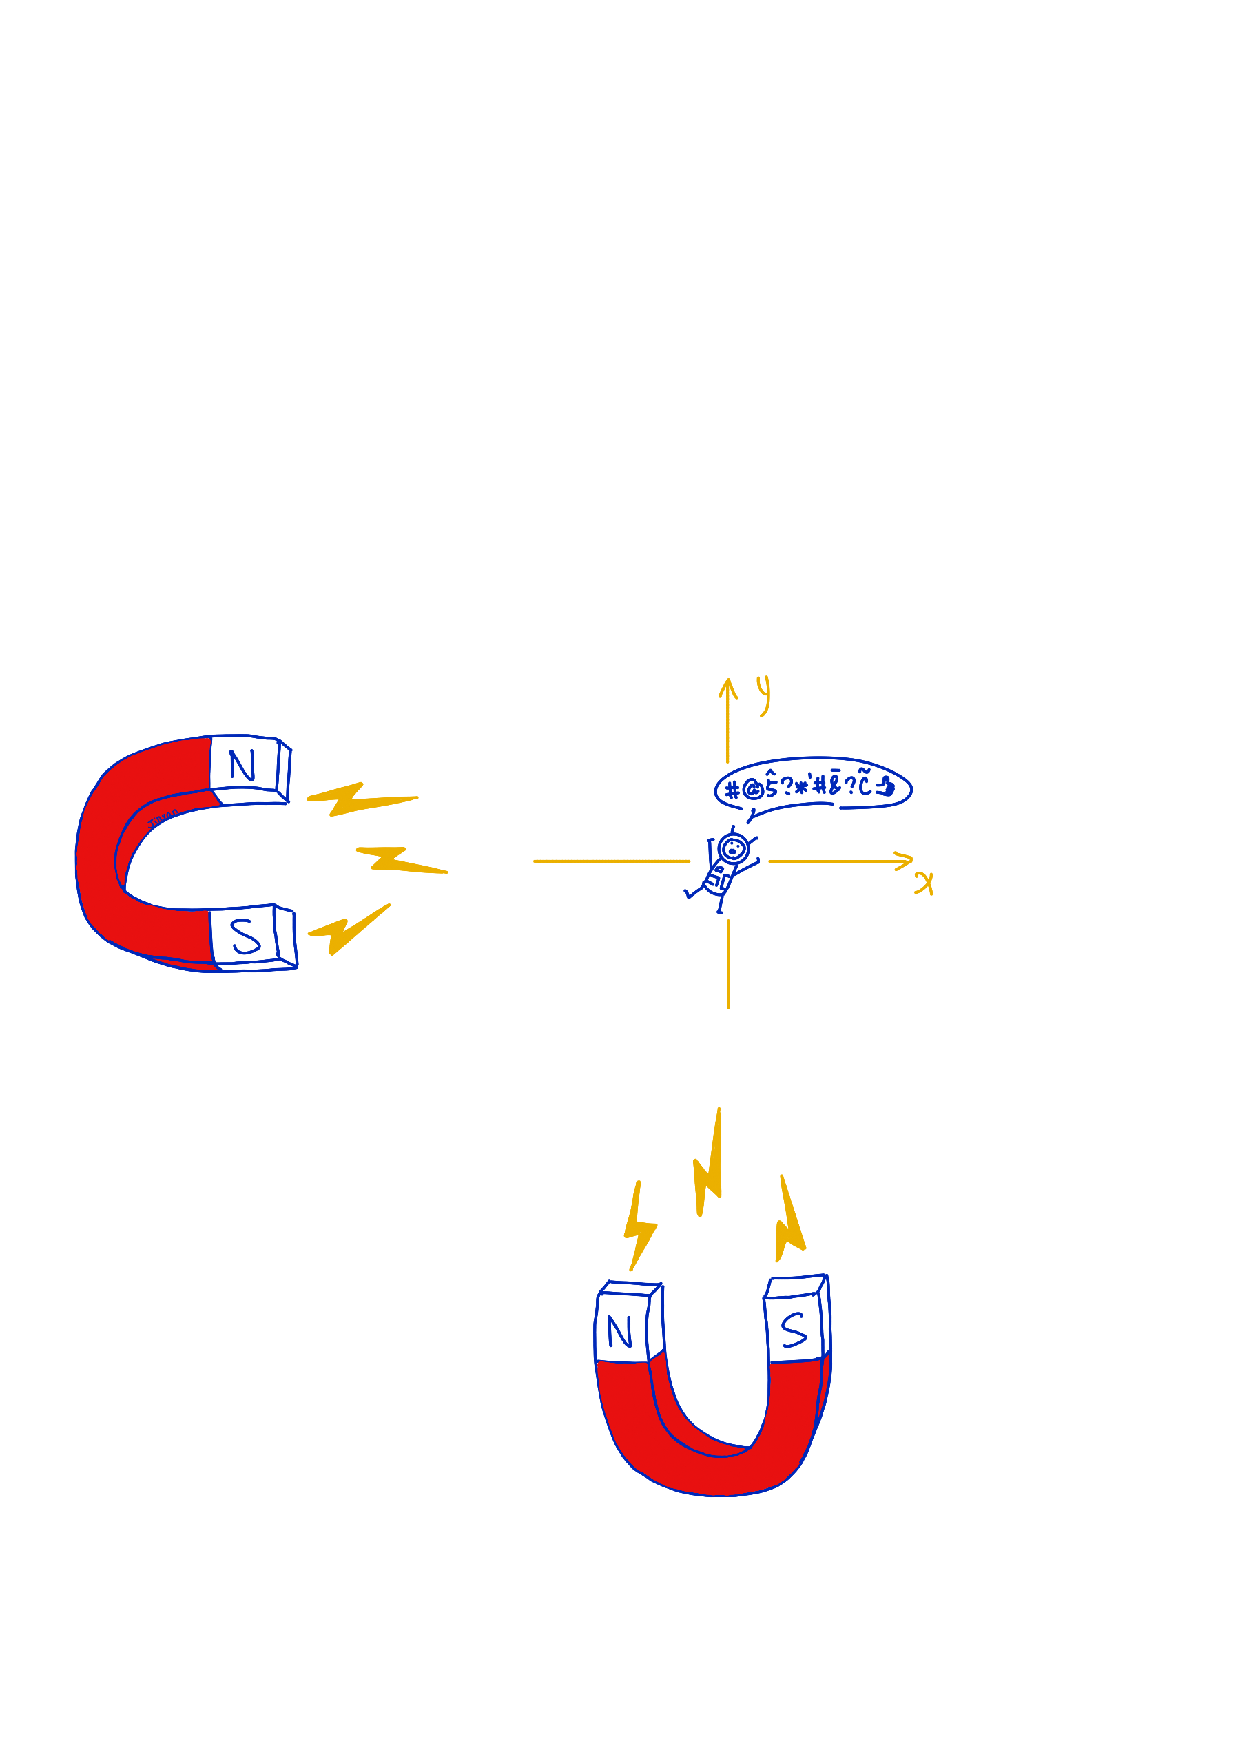
\includegraphics[scale=0.65]{magnet}
\end{center}



\newpage
\section*{Problem 1}
(a) The force has magnitude $F_q=2$\,N and points at an angle $\theta=45^\circ$ measured from the positive $x$-direction. Using the formulas given in the problem, we find its $x$- and $y$-components separately,
\begin{align*}
F_{q,x} &= F_q\cos(\theta) = (2\,\text{N})\cos(45^\circ)
= (2\,\text{N})\frac{1}{\sqrt{2}} = \sqrt{2}\,\text{N}\,,\\
F_{q,y} &= F_q\sin(\theta) = (2\,\text{N})\sin(45^\circ)
= (2\,\text{N})\frac{1}{\sqrt{2}} = \sqrt{2}\,\text{N}\,.
\end{align*}
Both components are positive because the force points up and to the right. Therefore, the component form of the electric force is
\begin{align*}
\vec{F}_q = (\sqrt{2},\ \sqrt{2})\,\text{N}
\approx (1.41,\ 1.41)\,\text{N}\,.
\end{align*}

\noindent (b) The gravitational force points directly downwards, so its component form is
\begin{align*}
\vec{F}_g = (0,\ -mg)\,.
\end{align*}
It has a zero $x$-component; thus, the gravitational force only affects the vertical motion of the charge, while the electric force that we have computed in part (a) affects both the vertical and horizontal motion of the charge. Mathematically, and this is also the key point of this problem, we need to sum the $x$- and $y$-components of the forces to get the net force acting on the object. The charge can move only in the positive $x$-direction when the net force has no $y$-component. Therefore, the upward $y$-component of the electric force must cancel the downward gravitational force. Adding the $y$-components and setting their sum equal to zero gives
\begin{align*}
F_{\text{net},y} &= F_{q,y}+F_{g,y}=\sqrt{2}\,\text{N}-mg =0\,,
\end{align*}
and thus 
$$mg = \sqrt{2}\,\text{N}\,.$$
Using $g=9.8$\,m/s$^2$, the mass is
\begin{align*}
m = \frac{\sqrt{2}\,\text{N}}{9.8\,\text{m/s}^2}
=0.144\,\text{kg}\,.
\end{align*}
After the $y$-components cancel, the remaining net force is $\vec{F}_{\text{net}}=(\sqrt{2},\,0)$\,N, which indeed points in the positive $x$-direction.\vspace{0.2cm}

\noindent (c) The charge $q_1$ is positive and $q_2$ is negative, so the two charges attract each other. This means that the electric force on $q_1$ must point from $q_1$ toward $q_2$. We already know that the force on $q_1$ points at $45^\circ$ from the positive $x$-direction. Therefore, $q_2$ must be located somewhere along the $45^\circ$ direction from $q_1$, which is up and to the right of $q_1$.\vspace{0.2cm}

\noindent (d) The magnitude of the electric force between two point charges is governed by Coulomb's law,
\begin{align*}
F_q = \frac{k|q_1q_2|}{r^2}\,,
\end{align*}
where $r$ is the distance between the two charges and $k=8.99\cdot 10^9$\,N\,m$^2$/C$^2$ is the Coulomb constant. Notice that this is a statement about the magnitude $F_q$ of the electric force. The equation does not give us information about the direction of such a force. Isolating $r$ from this equation, we obtain
\begin{align*}
r &= \sqrt{\frac{k|q_1q_2|}{F_q}}\,.
\end{align*}
Now we plug in $F_q=2$\,N, $q_1=1$\,C, and $q_2=-5$\,C,
\begin{align*}
r &= \sqrt{\frac{(8.99\cdot 10^9\,\text{N}\,\text{m}^2/\text{C}^2)|(1\,\text{C})(-5\,\text{C})|}{2\,\text{N}}}\\
&=\sqrt{2.2475\cdot 10^{10}\,\text{m}^2}
=1.50\cdot 10^5\,\text{m}\,.
\end{align*}
Therefore, the distance between $q_1$ and $q_2$ is approximately $1.50\cdot 10^5$\,m, or $150$\,km. The large distance comes from the unusually large charges given in the problem.\vspace{0.2cm}

\noindent (e) From Newton's third law, the electric force that $q_1$ exerts on $q_2$ has the same magnitude as the force that $q_2$ exerts on $q_1$, but points in the opposite direction. In component form,
\begin{align*}
\vec{F}_{1\text{ on }2} = -\vec{F}_{2\text{ on }1}
=-(\sqrt{2},\ \sqrt{2})\,\text{N}
=(-\sqrt{2},\ -\sqrt{2})\,\text{N}\,.
\end{align*}
Its magnitude is
\begin{align*}
|\vec{F}_{1\text{ on }2}| = \sqrt{(-\sqrt{2})^2+(-\sqrt{2})^2}
=\sqrt{4}\,\text{N}=2\,\text{N}\,.
\end{align*}
Both components are negative, so this force points down and to the left. Its direction is $225^\circ$ measured counterclockwise from the positive $x$-direction (equivalently, $45^\circ$ below the negative $x$-direction). Thus, the electric forces on the two charges have equal magnitudes and opposite directions, as expected.

\section*{Problem 2}
The net force that Jinyan experiences is 
\begin{align*}
\vec{F}_{\text{net}} = \vec{F}_1 + \vec{F}_2 = (-1000,\ -100) \,\text{N}\,.
\end{align*}
Notice here, we add the forces component-wise, and they have directions (to the left is negative in the $x$-direction, and downwards is negative in the $y$-direction, hence the negative signs). \underline{Never mix the $x$- and $y$-components; they should be treated independently}.\\

Now using Newton's second law, 
\begin{align*}
\vec{a} = \frac{\vec{F}_{\text{net}}}{m}= \left(-\frac{1000}{100}, \frac{-100}{100}\right) \,\text{m/s}^2 = (-10, -1) \,\text{m/s}^2\,.
\end{align*}
We see that $\vec{a}$ is a constant because $\vec{F}_{\text{net}}$ is a constant (in the problem we say the forces are constant throughout my journey). Therefore we can apply the kinematic equations (which require constant acceleration) for describing my motion in space. We have $a_x = -10$\,m/s$^2$ and $a_y = -1$\,m/s$^2$ as we just computed. The problem says I start at rest, thus $v_{0,x} = v_{0,y} = 0$\,m/s. Since I start at the origin, $x_0 = y_0 = 0$\,m. Assembling everything, 
\begin{align*}
y = \frac{1}{2}a_y t^2 + v_{0,y} t + y_0 = -0.5 t^2 \,,\qquad
x = \frac{1}{2}a_x t^2 + v_{0,x} t + x_0 = -5 t^2 \,.
\end{align*}
Therefore, my position vector after $t$ seconds is 
\begin{align*}
\vec{x} = (-5 t^2,\ -0.5 t^2)\,.
\end{align*}

\vspace*{\fill}
\noindent I like to include pictures at the end to show off places I have been to :)\\
\begin{center}
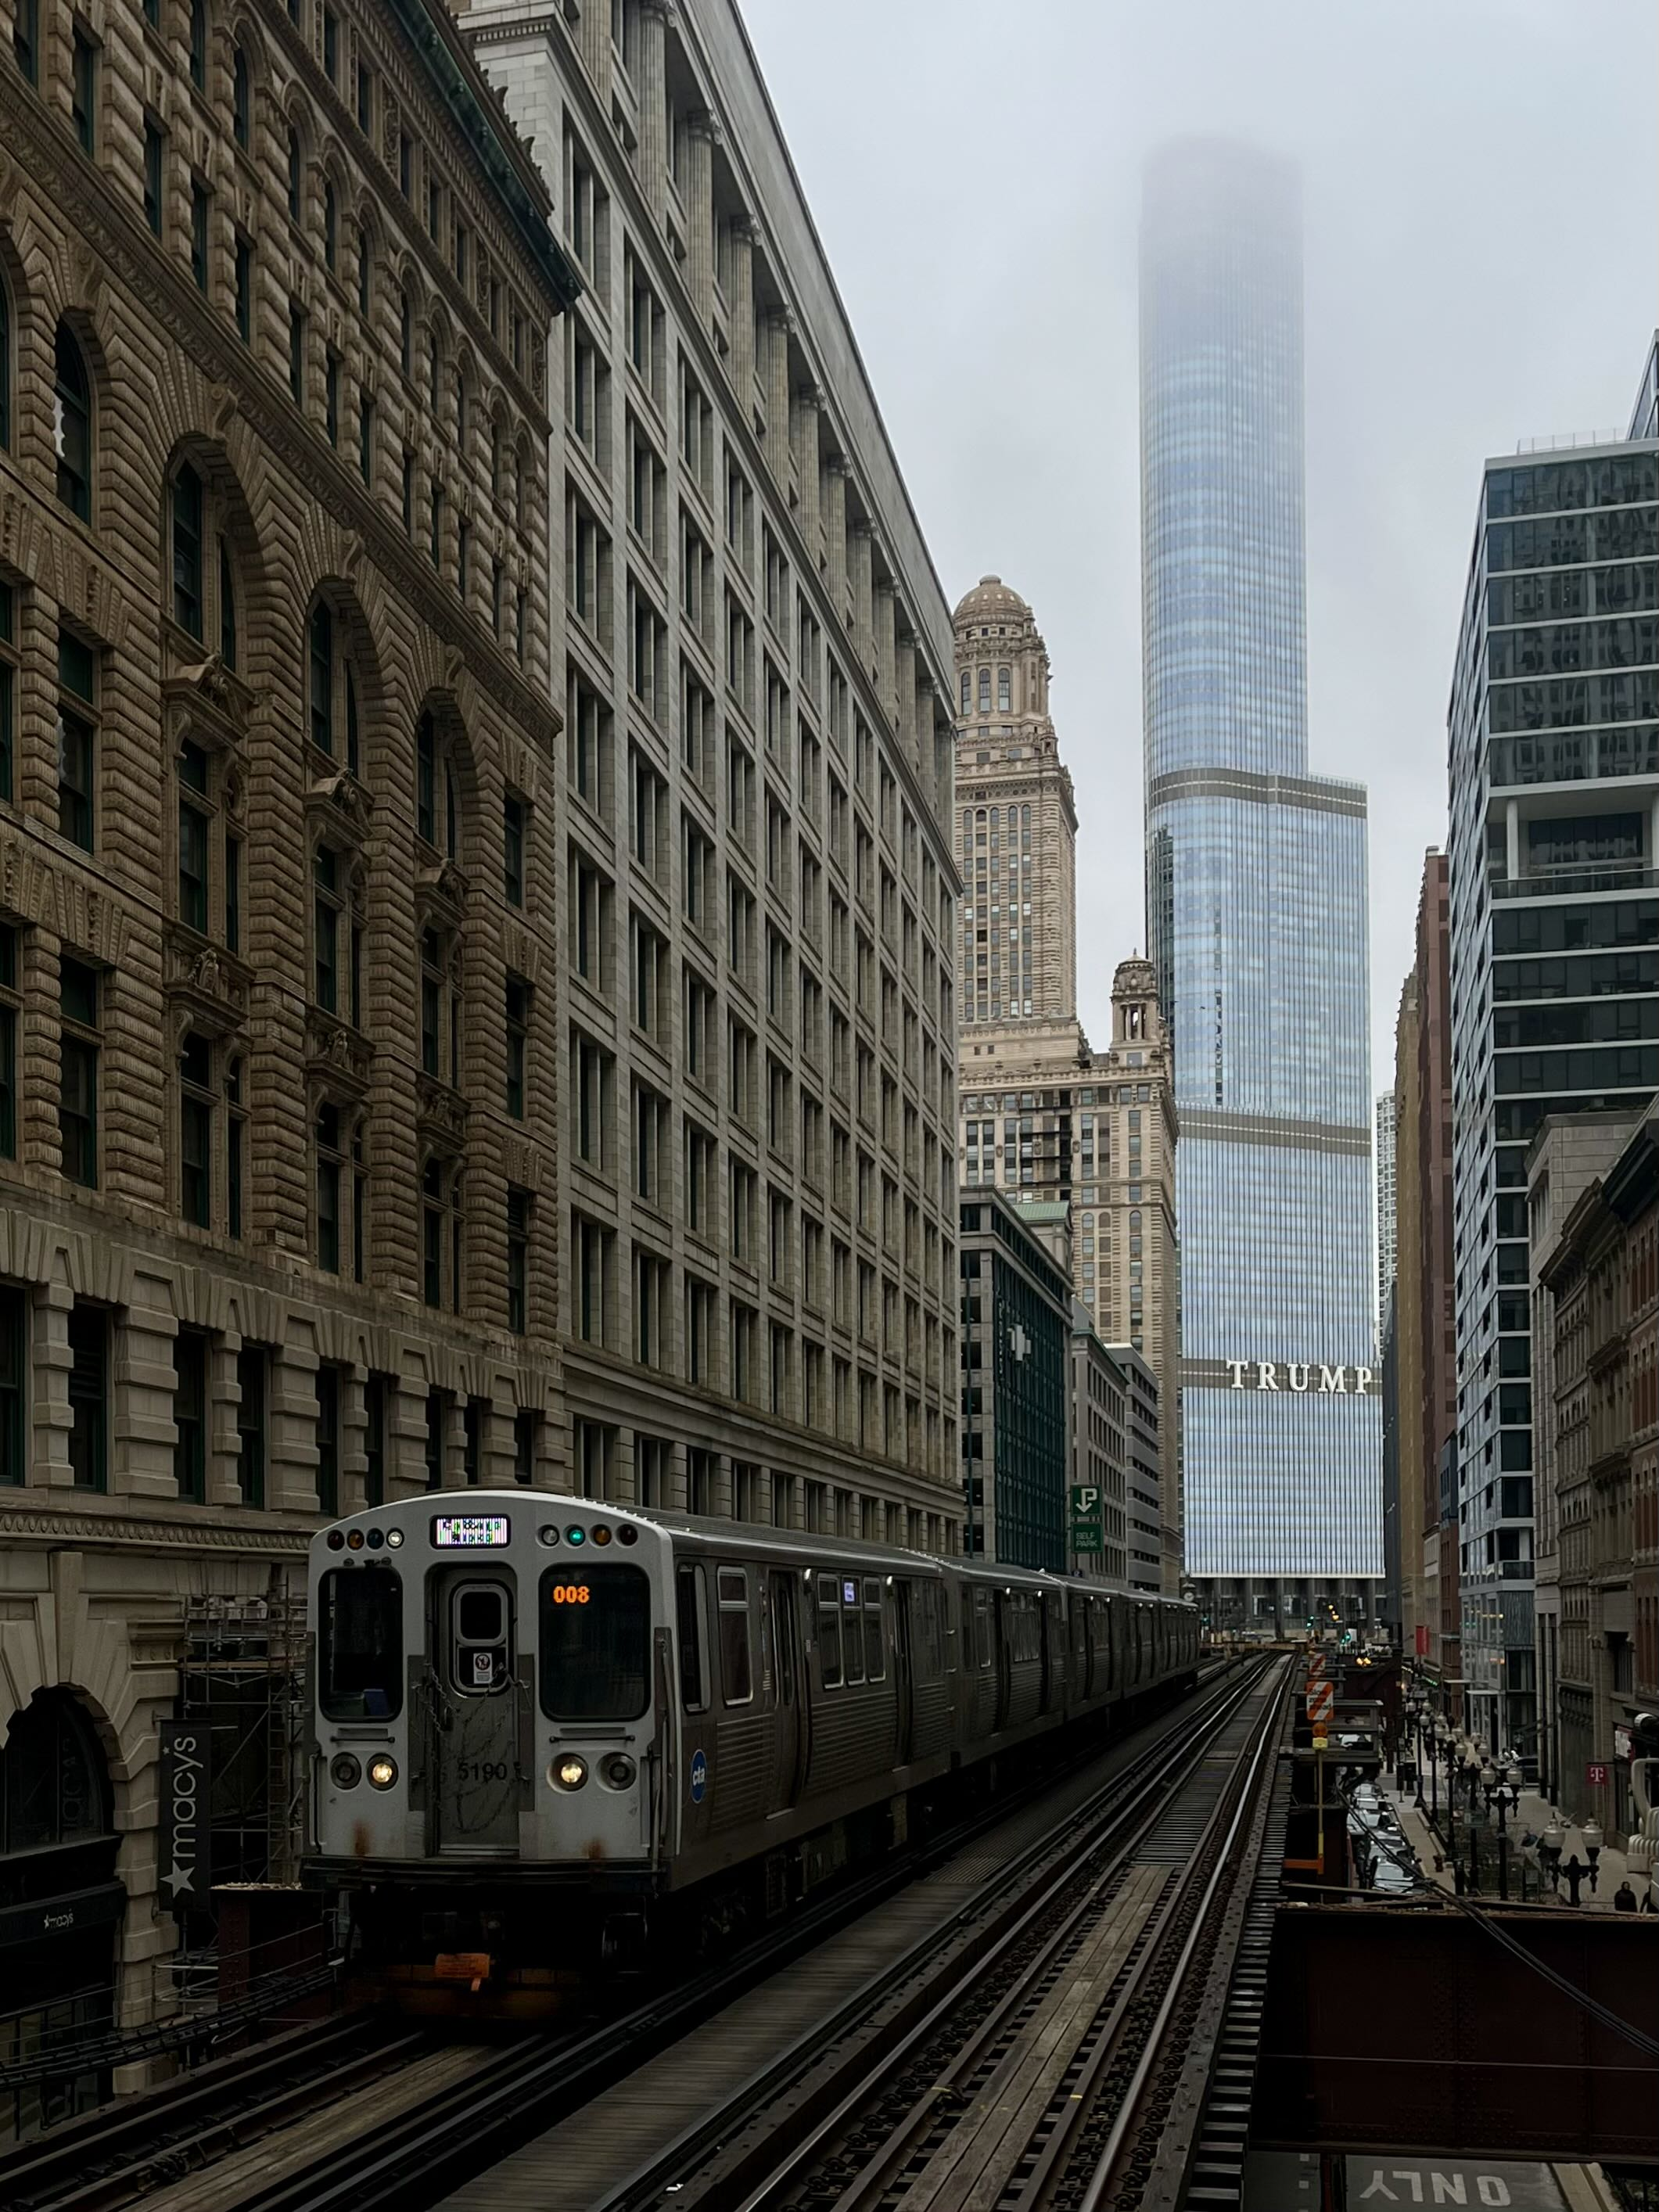
\includegraphics[scale=0.15]{IMG_1510.jpg}\\
\hfill\break
Downtown Chicago, pictured in March 2026. 
\end{center}


\end{document}
